%---------------------------------------------------------------------------
%	Packages
%---------------------------------------------------------------------------
\documentclass[twocolumn]{article}
\usepackage[bottom]{footmisc}
\usepackage[affil-it]{authblk}
\usepackage{amsmath}
\usepackage{setspace}
\usepackage{url}
\usepackage{amsthm}
\usepackage{tikz}
\usetikzlibrary{shapes.geometric, arrows}
\usetikzlibrary{decorations.pathreplacing}
\usetikzlibrary{calc}
\usepackage{pgfplots}
\usepgfplotslibrary{units}
\usepackage{indentfirst}
\usepackage{gensymb}
\pgfplotsset{compat=1.10}
\usepackage{amsmath,amsfonts,amssymb}
\usepackage{braket}
\usepackage{tikz}
\usetikzlibrary{shapes.geometric, arrows}
\usetikzlibrary{decorations.pathreplacing}
\usetikzlibrary{decorations.pathmorphing}
\usetikzlibrary{decorations.markings}
\usepackage{pgfplots}
\usepackage{pgf}
\usepackage{fancyhdr}
\usepgfplotslibrary{units}
\pgfplotsset{compat=1.10}
\usepgfplotslibrary{units}
\usepackage{tkz-euclide}
\usetkzobj{all}
\usepackage{xcolor}
\usepackage{graphicx}
\usetikzlibrary{arrows.meta}
\tikzset{>=Stealth}
\tikzset{snake it/.style={decorate, decoration=snake}}
\graphicspath{{Figures/}}
%---------------------------------------------------------------------------
%	Header and footer
%---------------------------------------------------------------------------
\pagestyle{fancy}
\lhead{\small{Improving Quantum Parameter Estimation}}
\chead{\small{T.J. Larrechea}}
\rhead{\small{Colorado Mesa University}}
%---------------------------------------------------------------------------
%	Title and Author
%---------------------------------------------------------------------------
\title{\textbf{Improving Quantum Parameter Estimation}}
\author{Taylor Larrechea\footnote{Electronic Address: \texttt{tjlarrechea@mavs.coloradomesa.edu.}} \\
    Colorado Mesa University \\
    Department of Physical and Environmental Sciences \\
    1100 North Avenue \\
    Grand Junction, CO 81501-3122}
\date{\today}
%---------------------------------------------------------------------------
%	Begin Document
%---------------------------------------------------------------------------
\begin{document}
\maketitle
%---------------------------------------------------------------------------
%	Abstract
%---------------------------------------------------------------------------
\begin{abstract}
Quantum parameter estimation, or metrology, is the method of which quantum mechanical systems are used as measuring devices to measure physical parameters. This paper discusses progress made in researching metrology for undergraduate research at Colorado Mesa University.
\end{abstract}
%---------------------------------------------------------------------------
%	Introduction
%---------------------------------------------------------------------------
\section*{Introduction}
Quantum parameter estimation deals with estimating physical parameters by using quantum mechanical systems as measuring devices. These systems can be used to measure physical parameters such as the strength of a magnetic field. In previous studies metrology has been studied to see if there are better approximation methods that exist. Particularly if using states such as entangled states enhance the estimation accuracy compared to other classical strategies \cite{D. Collins}. The research that is being reported in this article covers a similar question about how to improve estimation accuracy, particularly by using multiple states at once. In the examination of mixed and pure states we become interested in measuring multiple states at once. When multiple states are measured in comparison to single states the question arises as to if product or entangled states yield a better estimation to physical parameters.
%---------------------------------------------------------------------------
%	Quantum Spin - 1/2 Systems
%---------------------------------------------------------------------------
\section*{Quantum Spin - 1/2 Particles}
We start with understanding what Spin - 1/2 Particles are. For example, take a particle that is being sent into a magnetic field. A particle that resides in a specific state, usually denoted by $\ket{\psi}$, can be subjected to a measurement influenced by a physical parameter. After the measurement is taken on the particle we can repeat this process hundreds of times to learn more about the probabilities of getting a specific measurement. Quantum physics tells us that the resulting measurement can come out to be either $S_{n+}=\hbar/2$ or $S_{n-}=-\hbar/2$. Both of these results will eventually add up to have a probability of one depending upon the original orientation of the particle in the given state $\ket{\psi}$.

When these experiments are repeated several times, that is subjecting a particle to a measurement, we begin to have a better understanding of the probability of either obtaining $\hbar/2$ or $-\hbar/2$ from our measurement. Using quantum mechanics we can then begin to state certain things about the state itself such as the angle $\theta$ and the angle $\phi$ from their respective axis'. The angles can be seen in Figure 1.
%--------------------------------------------------
%	Figure 1
%--------------------------------------------------
\begin{figure}[htbp]
\begin{center}
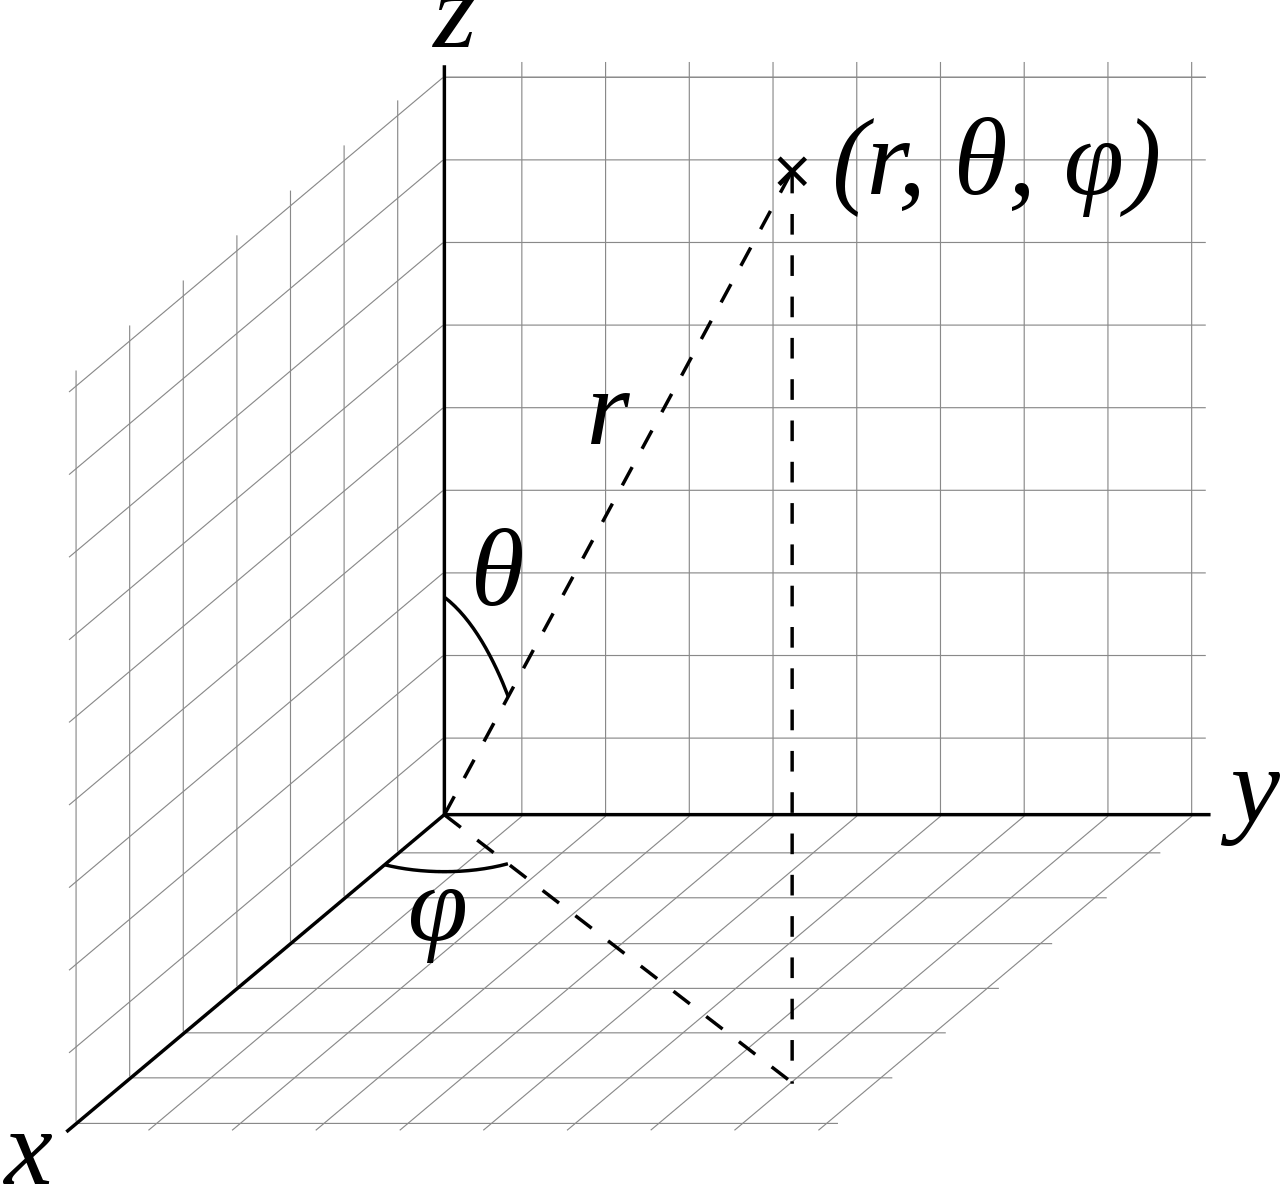
\includegraphics[width=0.75\linewidth]{Spherical-Coordinate-System.png}
\caption{Generic Representation of 3D Spherical Coordinate System.}
\end{center}
\end{figure}
\newline
\newline
Particles are subject to being measured can have any orientation with any value of $\theta$ or $\phi$. Typically these particles that are being described are spin - $1/2$ particles. We will now begin to discuss spin - $1/2$ particles that are present in a magnetic field.

There are ways that we can describe these spin - $1/2$ systems with the language of Quantum Mechanics. Conversely Quantum Mechanics can be described in the language of Linear Algebra, specifically in this case with bras and kets. These spin - $1/2$ systems can be described with the ket 
%--------------------------------------------------
%	Equation (1)
%--------------------------------------------------
\begin{equation} \label{eq:1}
\ket{\psi}=a_{+}\ket{+\hat{z}}+a_{-}\ket{-\hat{z}}
\end{equation}
where $a_{+}$ and $a_{-}$ are normalization constants. When we subject these particles to a measurement in either the $x, \hspace{1pt} y$, or $z$ direction we have the possibility of getting one of two outcomes, either $+\hbar/2$ or $-\hbar/2$. This scheme can be seen in Figure 2. 
\newpage
%--------------------------------------------------
%	Figure 2
%--------------------------------------------------
\begin{figure}[htpb]
\begin{center}
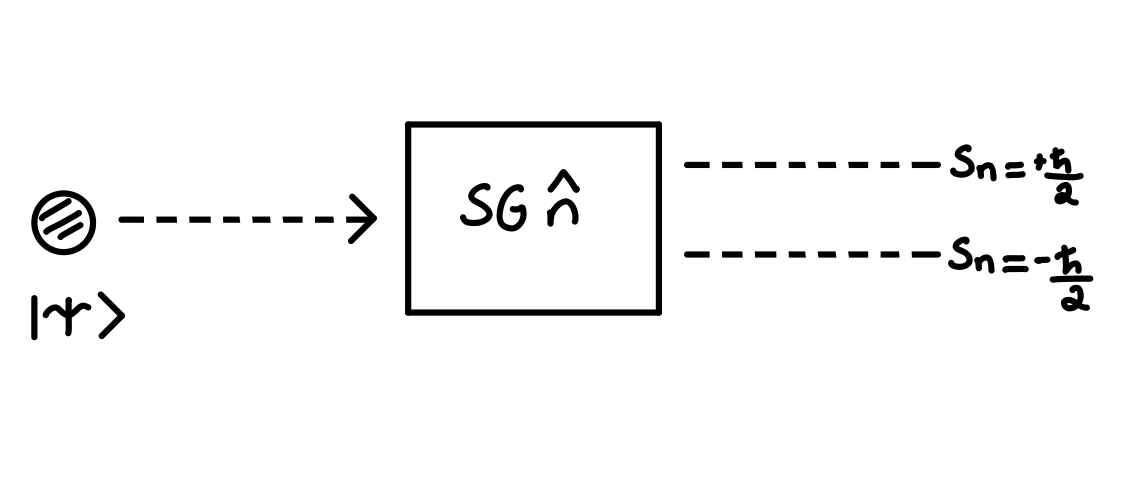
\includegraphics[width=0.90\linewidth]{SG-Measurement.PNG}
\caption{Schematic of SG Measurement.}
\end{center}
\end{figure}
Figure 2 encompasses a generic state $\hat{n}$ which can either be the $x, \hspace{1pt} y$, or $z$ direction. These states can represent the $x, \hspace{1pt} y$, or $z$ direction by knowing $\theta$ and $\phi$ for whatever particle we are interested in measuring. These states can be calculated by
%--------------------------------------------------
%	Equations (2)
%--------------------------------------------------
\begin{equation} \label{eq:2}
\ket{+\hat{n}}=\cos{(\theta/2)}\ket{+\hat{z}}+e^{i\phi}\sin{(\theta/2)}\ket{-\hat{z}}
\end{equation}
and
%--------------------------------------------------
%	Equations (3)
%--------------------------------------------------
\begin{equation} \label{eq:3}
\ket{-\hat{n}}=\sin{(\theta/2)}\ket{+\hat{z}}-e^{i\phi}\cos{(\theta/2)}\ket{-\hat{z}}.
\end{equation}
Every direction, whether it is the $x$, $y$, or $z$ has a positive and negative orientation. Equation (\ref{eq:2}) represents how to calculate the positive direction and equation (\ref{eq:3}) represents how to calculate the negative direction. Along with equation (\ref{eq:2}) representing the positive direction of a particles orientation, equation (\ref{eq:2}) represents the state in which we would measure to obtain $\hbar/2$ with some degree of certainty. The same can be said for equation (\ref{eq:3}) but this equation represents the direction we would measure against to obtain $-\hbar/2$ with some degree of certainty. When these particles are subjected to a measurement they will be reoriented from their original orientation.

These particles can be measured against other specific directions. Mathematically this calculation is 
%--------------------------------------------------
%	Equation (4)
%--------------------------------------------------
\begin{equation} \label{eq:4}
\bra{\pm n}\ket{\pm m}
\end{equation}
which is how we determine how states are affected under measurements. Once these states are known we can also calculate the probabilities of getting $+\hbar/2$ and $-\hbar/2$. Quantum theory tells us that we can calculate these probabilities by
%--------------------------------------------------
%	Equation (5)
%--------------------------------------------------
\begin{equation} \label{eq:5}
\text{Prob}=|\bra{\pm\hat{n}}\ket{\psi}|^2
\end{equation}
where the probabilities of getting $+\hbar/2$ and $-\hbar/2$ must add up to be 1. The state $\ket{\psi}$ can be written in the form of equation (\ref{eq:1}) where the components $a_+$ and $a_-$ must satisfy $|a_+|^2+|a_-|^2=1$.

It is more conventional to write equations (\ref{eq:2}) and (\ref{eq:3}) as in $\ket{0}$ and $\ket{1}$ notation. Precisely, these equations are
%--------------------------------------------------
%	Equation (6)
%--------------------------------------------------
\begin{equation} \label{eq:6}
\ket{+\hat{n}}=\cos{(\theta/2)}\ket{0}+e^{i\phi}\sin{(\theta/2)}\ket{1}
\end{equation}
and
%--------------------------------------------------
%	Equation (7)
%--------------------------------------------------
\begin{equation} \label{eq:7}
\ket{-\hat{n}}=\sin{(\theta/2)}\ket{0}-e^{i\phi}\cos{(\theta/2)}\ket{1}.
\end{equation}
The notation that is denoted in equation (\ref{eq:6}) and (\ref{eq:7}) is what will be used throughout the rest of this paper to described spin-1/2 particles with specific states.
%---------------------------------------------------------------------------
%	Entangled and Product States
%---------------------------------------------------------------------------
\section*{Entangled and Product States}
Product and entangled states are states that represent multiple particles. Product states are two states of which that can be separated into two separate individual states. Entangled states are states that involve two states that cannot be separated such that each individual state can be recognized.

Within these multiple particle states there are a set of generic states. These generic states are $\ket{0}\ket{0}$, $\ket{0}\ket{1}$, $\ket{1}\ket{0}$, and $\ket{1}\ket{1}$. In these generic states we have a combination of particles either being positive or negative. The $\ket{0}$'s are positive and the $\ket{1}$'s are negative. There are states of which are entangled or product states where we can take measurements and calculate probabilities. The way these probabilities are calculated is
%--------------------------------------------------
%	Equation (8)
%--------------------------------------------------
\begin{equation}\label{eq:8}
\text{Prob}=|\bra{n_{0,1}}\bra{n_{0,1}}\ket{\psi}|^2
\end{equation}
where $\bra{n_0}=\bra{0}$ and $\bra{n_1}=\bra{1}$. 

These states can be in the state of superposition. Take for instance the state
%--------------------------------------------------
%	Equation (9)
%--------------------------------------------------
\begin{equation}\label{eq:9}
\ket{\psi}=\frac{1}{2}\big(\ket{0}\ket{0}+\ket{0}\ket{1}-\ket{1}\ket{0}-\ket{1}\ket{1}\big)
\end{equation}
which is an example of a product state. Equation (\ref{eq:9}) can be written as a combination of states such that
%--------------------------------------------------
%	Equation (10)
%--------------------------------------------------
\begin{equation}\label{eq:10}
\ket{\psi}=\ket{\psi_A}\ket{\psi_B}.
\end{equation}
Just as equation (\ref{eq:9}) represents a product state, entangled states can be written in a similar fashion. An example of an entangled state is
%--------------------------------------------------
%	Equation (11)
%--------------------------------------------------
\begin{equation}\label{eq:11}
\ket{\psi}=\frac{1}{2}\big(\ket{0}\ket{0}+\ket{0}\ket{1}+\ket{1}\ket{0}-\ket{1}\ket{1}\big).
\end{equation}
Equation (\ref{eq:11}) cannot be separated into two separate states in the form of equation (\ref{eq:10}) and this is what makes the state entangled. No matter how hard we try, we cannot come up with a $\ket{\psi_A}$ and $\ket{\psi_B}$ for this specific entangled state.

When these product and entangled states are subjected to measurements, it is typical that one particle undergoes an evolution where the other particle is left alone. This process ends up being more accurate than measuring a single particle alone. It can be shown later on that measuring parameters with entangled states is a more accurate method for estimating parameters than that even of product states.
%---------------------------------------------------------------------------
%	Unitary Operators
%---------------------------------------------------------------------------
\section*{Unitary Operators}
We now move on to investigating unitary operators and how they make states evolve. To have a better understanding of how unitary operators work, Figure 3 depicts how they make states evolve.
%--------------------------------------------------
%	Figure 3
%--------------------------------------------------
\begin{figure}[htpb]
\begin{center}
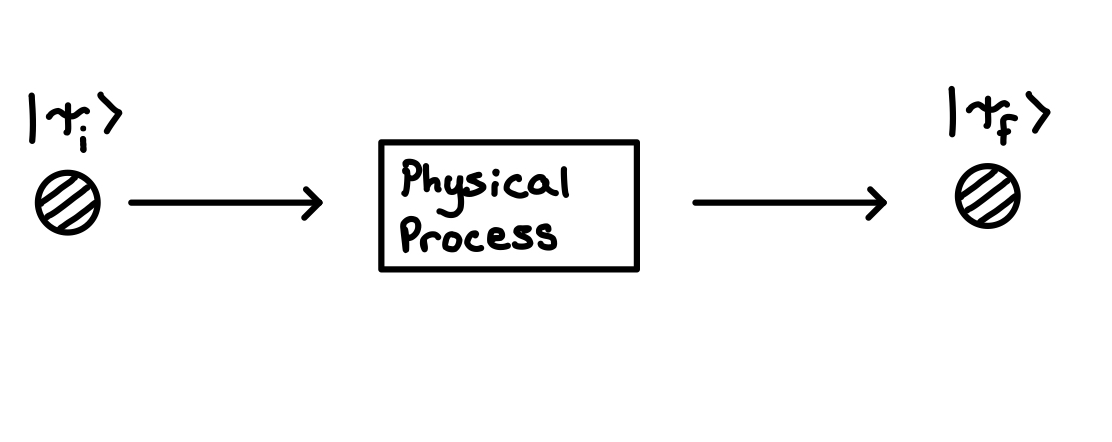
\includegraphics[width=0.90\linewidth]{Unitary-Operator.PNG}
\caption{Schematic of Unitary Operator.}
\end{center}
\end{figure}\\
In short, unitary operators take a state and change and reorient it to a different state. These unitary operators can be symbolic of how a particle is affected when it enters a magnetic field. Mathematically this evolution can be calculated by
%--------------------------------------------------
%	Equation (12)
%--------------------------------------------------
\begin{equation}\label{eq:12}
\ket{\psi_f}=\hat{U}\ket{\psi_i}
\end{equation}
where $\hat{U}^{\intercal}\hat{U}$ must be true. There are special unitary operators called Pauli operators and there is one Pauli Operator for the $x$, $y$, and $z$-direction. The $x$-direction Pauli operator is
%--------------------------------------------------
%	Equation (13)
%--------------------------------------------------
\begin{equation}\label{eq:13}
\hat{\sigma}_x=
\begin{pmatrix}
0 & 1 \\
1 & 0
\end{pmatrix}
\end{equation}
and the $y$-direction
%--------------------------------------------------
%	Equation (14)
%--------------------------------------------------
\begin{equation}\label{eq:14}
\hat{\sigma}_y=
\begin{pmatrix}
0 & -i \\
i & 0
\end{pmatrix}
\end{equation}
and lastly the $z$-direction is
%--------------------------------------------------
%	Equation (15)
%--------------------------------------------------
\begin{equation}\label{eq:15}
\hat{\sigma}_z=
\begin{pmatrix}
1 & 0 \\
0 & -1
\end{pmatrix}.
\end{equation}
These Pauli operators will be referenced later in this paper and instead of writing out a matrix every time they are mentioned we will just refer to these equations for simplicity sakes. These unitary operators can be acted on particles in certain states and be used to determine how the states reorient themselves after the interaction.

Consider the unitary operator
%--------------------------------------------------
%	Equation (16)
%--------------------------------------------------
\begin{equation}\label{eq:16}
\hat{U}=
\begin{pmatrix}
1 & 0 \\
0 & -1
\end{pmatrix}
\end{equation}
which is the $\hat{\sigma}_z$. We can now examine how this unitary operator affects specific initial states. The effects of the unitary operator represented by equation (\ref{eq:16}) acting on specific initial states can be seen in Table 1. 
%--------------------------------------------------
%	Table 1
%--------------------------------------------------
\begin{table}[h!]
\begin{center}
\begin{tabular}{ |c|c| }
\hline $\ket{\psi_i}$& $\hat{U}\ket{\Psi_i}=\ket{\psi_f}$ \\
\hline $\ket{0}$& $\ket{0}$\\
\hline $\frac{1}{\sqrt{2}}\big(\ket{0}+\ket{1}\big)$& $\frac{1}{\sqrt{2}}\big(\ket{0}-\ket{1}\big)$\\
\hline $\frac{1}{2}\big(\ket{0}+i\ket{1}\big)$& $\frac{1}{\sqrt{2}}\big(\ket{0}-i\ket{1}\big)$\\
\hline
\end{tabular}
\caption{Effect of the $\hat{\sigma}_z$ Pauli Operator Acting on Spin-1/2 Particles.}
\end{center}
\end{table} \\
When the unitary operator in equation (\ref{eq:16}) acts on the spin-1/2 particles in Table 1 it subsequently flips the direction that it was originally oriented in. These shifts can be seen in Table 2.
\newpage
%--------------------------------------------------
%	Table 2
%--------------------------------------------------
\begin{table}[h!]
\begin{center}
\begin{tabular}{ |c|c|c|c| }
\hline $\ket{\psi_i}$ $(\theta_i)$& $\ket{\psi_i}$ $(\phi_i)$& $\ket{\psi_f}$ $(\theta_f)$& $\ket{\psi_f}$ $(\psi_f)$ \\
\hline 0 & 0 & 0 & 0 \\
\hline $\pi/2$ & 0 & $\pi/2$ & $\pi$ \\
\hline $\pi/2$ & $\pi/2$ & $\pi/2$ & $3\pi/2$ \\
\hline
\end{tabular}
\caption{The Effect of the $\sigma_z$ Pauli Operator on the $\theta$ and $\phi$ Angles.}
\end{center}
\end{table} 
The rows in Table 2 are angles in radians for each state previously mentioned in Table 1. It can be observed that the $\theta$ angle is not affected by the unitary operator acting on the spin-1/2 particles in these specific original states. Instead, when the spin-1/2 particle is originally oriented in the $x$ or $y$-direction the $\phi$ angle is reoriented by an angle of $\pi$. This is because this unitary operator is causing a rotation for these particles about the $z$ axis. This rotation about the $z$ axis is why the particle that is originally oriented in the $z$ direction (The first row of Table 2) is unaffected by this unitary operator in equation (\ref{eq:16}).
%---------------------------------------------------------------------------
%	Unitary Operators With a Parameter
%---------------------------------------------------------------------------
\section*{Unitary Operators With a Parameter}
Unitary operators can also be dependent upon parameters. Take for instance the unitary operator
%--------------------------------------------------
%	Equation (17)
%--------------------------------------------------
\begin{equation}\label{eq:17}
\hat{U}(\lambda)=
\begin{pmatrix}
e^{-i\lambda/2} & 0 \\
0 & e^{i\lambda/2}
\end{pmatrix}
\end{equation}
which is dependent upon the parameter $\lambda$. When this unitary operator acts on states it will produce a final state after that is also dependent upon a parameter. The results of this unitary operator acting on specific spin-1/2 states can be seen in Table 3. \\
\newpage
%--------------------------------------------------
%	Table 3
%--------------------------------------------------
\begin{table}[h!]
\begin{center}
\begin{tabular}{ |c|c| }
\hline $\ket{\psi_i}$& $\hat{U}\ket{\Psi_i}=\ket{\psi_f}$ \\
\hline $\ket{0}$& $e^{-i\lambda/2}\ket{0}$\\
\hline $\frac{1}{\sqrt{2}}\big(\ket{0}+\ket{1}\big)$& $\frac{1}{\sqrt{2}}\big(e^{-i\lambda/2}\ket{0}+e^{i\lambda/2}\ket{1}\big)$\\
\hline $\frac{1}{5}\big(4\ket{0}+3\ket{1}\big)$& $\frac{1}{5}\big(4e^{-i\lambda/2}\ket{0}+3e^{i\lambda/2}\ket{1}\big)$\\
\hline
\end{tabular}
\caption{Effect of the Unitary Operator $\hat{U}(\lambda)$ on Initial Spin-1/2 Particle States.}
\end{center}
\end{table} 
Using the $\ket{\psi_f}$ states and comparing them with $\ket{\psi_i}$ we can see how the unitary operator affected the original state. These effects can be seen in Table 4.
%--------------------------------------------------
%	Table 4
%--------------------------------------------------
\begin{table}[h!]
\begin{center}
\begin{tabular}{ |c|c|c|c| }
\hline $\ket{\psi_i}$ $(\theta_i)$& $\ket{\psi_i}$ $(\phi_i)$& $\ket{\psi_f}$ $(\theta_f)$& $\ket{\psi_f}$ $(\phi_f)$ \\
\hline 0 & 0 & 0 & 0 \\
\hline $\pi/2$ & 0 & $\pi/2$ & $\lambda$ \\
\hline $73.7\degree$ & $0$ & $73.7\degree$ & $\lambda$ \\
\hline
\end{tabular}
\caption{Effect of the Unitary Operator $\hat{U}(\lambda)$ on the $\theta$ and $\phi$ Angles.}
\end{center}
\end{table} \\

Similar to unitary operators, Pauli operators all follow a certain list of rules. The first rule is that any Pauli operator in any direction multiplied with itself will yield the identity matrix. Mathematically this can be interpreted as
%--------------------------------------------------
%	Equation (18)
%--------------------------------------------------
\begin{equation}\label{eq:18}
\hat{\sigma_n}^2=\hat{I}
\end{equation}
where $n$ is either the $x$, $y$, or $z$-direction. The next rule is for when we multiply separate Pauli operators in different directions we get something of the form $i\sigma_n$. Particularly these rules are
%--------------------------------------------------
%	Equation (19)
%--------------------------------------------------
\begin{equation}\label{eq:19}
\hat{\sigma}_x\hat{\sigma}_y=i\hat{\sigma}_z,
\end{equation}
%--------------------------------------------------
%	Equation (20)
%--------------------------------------------------
\begin{equation}\label{eq:20}
\hat{\sigma}_y\hat{\sigma}_z=i\hat{\sigma}_x,
\end{equation}
and
%--------------------------------------------------
%	Equation (21)
%--------------------------------------------------
\begin{equation}\label{eq:21}
\hat{\sigma}_z\hat{\sigma}_x=i\hat{\sigma}_y.
\end{equation}
The last rule is
%--------------------------------------------------
%	Equation (22)
%--------------------------------------------------
\begin{equation}\label{eq:22}
\sigma^2=\big(n_x^2+n_y^2+n_z^2\big)\hat{I}
\end{equation}
where $n_x$, $n_y$, and $n_z$ are all constants. With these rules we can drastically simplify our math when dealing with these Pauli operators.

The last thing we did was calculate matrix exponentials. Using the formula
%--------------------------------------------------
%	Equation (23)
%--------------------------------------------------
\begin{equation}\label{eq:23}
e^{-i\lambda\hat{\sigma}_n}=\cos{(\lambda)}\hat{I}-i\sin{(\lambda)}\hat{\sigma}
\end{equation}
we can calculate matrix exponentials in any direction we choose. For example, $e^{-i\lambda\hat{\sigma}_z}$ can be written in the matrix form
%--------------------------------------------------
%	Equation (24)
%--------------------------------------------------
\begin{equation}\label{eq:24}
e^{-i\lambda\hat{\sigma}_z}=
\begin{pmatrix}
\cos{(\lambda)}-i\sin{(\lambda)} & 0 \\
0 & \cos{(\lambda)}+i\sin{(\lambda)}
\end{pmatrix}.
\end{equation}
But it is easier most of the time to represent this matrix with $e^{-i\lambda\hat{\sigma}_z}$.
%---------------------------------------------------------------------------
%	Two Qubit Unitary Operators
%---------------------------------------------------------------------------
\section*{Two Qubit Unitary Operators}
In the presence of two qubits interacting the evolution has to be described by an operator that acts on a pair of qubits. A popular qubit unitary that behaves in this manner is called the controlled not matrix. This matrix is abbreviated by $U_{\tiny{CNOT}}$ and is
%--------------------------------------------------
%	Equation (25)
%--------------------------------------------------
\begin{equation} \label{eq:25}
U_{\tiny{CNOT}}=
\left(\begin{array}{cccc}
1 & 0 & 0 & 0 \\
0 & 1 & 0 & 0 \\
0 & 0 & 0 & 1 \\
0 & 0 & 1 & 0 \\
\end{array}\right)
\end{equation}
and has the ability to change a product state to an entangled state for given initial states. The evolution of specific states under the controlled not unitary operator can be seen in Table 5.
%--------------------------------------------------
%	Table 5
%--------------------------------------------------
\begin{table}[h!]
\begin{center}
\begin{tabular}{ |c|c|c| }
\hline $\ket{\psi_0}$ & $\hat{U_{CNOT}}\ket{\Psi_0}=\ket{\psi}$ & Result \\
\hline $\frac{1}{\sqrt{2}}(\ket{0}\ket{0}+\ket{0}\ket{1})$ & $\frac{1}{\sqrt{2}}(\ket{0}\ket{0}+\ket{0}\ket{1})$ & Prod. \\
\hline $\frac{1}{\sqrt{2}}(\ket{0}\ket{0}+\ket{1}\ket{0})$ & $\frac{1}{\sqrt{2}}(\ket{0}\ket{0}+\ket{1}\ket{1})$ & Ent. \\
\hline $\frac{1}{\sqrt{2}}(\ket{0}\ket{0}+\ket{1}\ket{1})$ & $\frac{1}{\sqrt{2}}(\ket{0}\ket{0}+\ket{1}\ket{0})$ & Prod. \\
\hline $\frac{1}{\sqrt{2}}(\ket{0}\ket{1}+\ket{1}\ket{0})$ & $\frac{1}{\sqrt{2}}(\ket{0}\ket{1}+\ket{1}\ket{1})$ & Prod. \\
\hline 
\end{tabular}
\caption{Effect of the Controlled Not Operator Acting on Original Product and Entangled States.}
\end{center}
\end{table} \\
As observed in Table 5, sometimes that controlled not operator converts a product state to an entangled state and vice versa. There are specific examples of where this does not happen.
%---------------------------------------------------------------------------
%	Density Operators
%---------------------------------------------------------------------------
\section*{Density Operators}
The next type of operator that we will examine is a density operator. We will specifically examine single qubits and the probabilities of their respective density operators. Suppose a single qubit has the density operator of
%--------------------------------------------------
%	Equation (26)
%--------------------------------------------------
\begin{equation} \label{eq:26}
\hat{\rho}=\frac{1}{2}
\begin{pmatrix}
1+r & 0 \\
0 & 1-r
\end{pmatrix}
\end{equation}
where we can calculate the probability of obtaining $\hbar/2$ and $-\hbar/2$ with certainty by
%--------------------------------------------------
%	Equation (27)
%--------------------------------------------------
\begin{equation} \label{eq:27}
\bra{\pm \hat{n}} \hat{\rho} \ket{\pm \hat{n}}.
\end{equation}
It should be noted that $0 \leq r \leq 1$. The probabilities of this measurement operator with $z$ and $x$-direction can be seen in Table 6.
%--------------------------------------------------
%	Table 6
%--------------------------------------------------
\begin{table}[h!]
\begin{center}
\begin{tabular}{ |c|c| }
\hline Direction & Probability \\
\hline $\bra{+\hat{z}}$ $\hat{\rho}$ $\ket{+\hat{z}}$ & $\frac{1+r}{2}$ \\
\hline $\bra{-\hat{z}}$ $\hat{\rho}$ $\ket{-\hat{z}}$ & $\frac{1-r}{2}$ \\
\hline $\bra{+\hat{x}}$ $\hat{\rho}$ $\ket{+\hat{x}}$ & $\frac{1}{2}$ \\
\hline $\bra{-\hat{x}}$ $\hat{\rho}$ $\ket{-\hat{x}}$ & $\frac{1}{2}$ \\
\hline
\end{tabular}
\caption{Probabilities of Measuring $\hbar/2$ and $-\hbar/2$ With the Density Operator in Equation (\ref{eq:26}) for the $z$ and $x$-Directions.}
\end{center}
\end{table} \\
One can construct a density operator by knowing the probabilities and the initial states of a specific measurement. Mathematically this is
%--------------------------------------------------
%	Equation (28)
%--------------------------------------------------
\begin{equation} \label{eq:28}
\hat{\rho}=a_1\ket{\psi_1}\bra{\psi_1}+a_2\ket{\psi_2}\bra{\psi_2}
\end{equation}
where $a$ is the probability and $\ket{\psi}$ is the state. For instance, if we know that the initial state is $\ket{0}$ with the probability of $q$ and $\ket{1}$ with the probability of $1-q$, the respective density operator $\hat{\rho}$ is
%--------------------------------------------------
%	Equation (29)
%--------------------------------------------------
\begin{equation} \label{eq:29}
\hat{\rho}=
\begin{pmatrix}
q & 0 \\
0 & 1-q
\end{pmatrix}.
\end{equation}

Another way of calculating the probability of a density operator is
%--------------------------------------------------
%	Equation (30)
%--------------------------------------------------
\begin{equation} \label{eq:30}
\text{Probability}=Tr[\hat{\rho}\hat{\rho_0}]
\end{equation}
where the trace of a matrix, $Tr$, is defined as the addition of the diagonals of a matrix. Where $\hat{\rho_0}$ is a density operator for a given direction. Take for instance the density operator
%--------------------------------------------------
%	Equation (31)
%--------------------------------------------------
\begin{equation} \label{eq:31}
\hat{\rho}=\frac{1}{2}
\begin{pmatrix}
1 & r \\
r & 1
\end{pmatrix}
\end{equation}
where we wish to calculate the probability of measuring $\hbar/2$ and $-\hbar/2$ with certainty for the $x$ and $y$-directions. The density operator for the positive $x$-direction is
%--------------------------------------------------
%	Equation (32)
%--------------------------------------------------
\begin{equation} \label{eq:32}
\hat{\rho}_{+x}=\frac{1}{2}
\begin{pmatrix}
1 & 1 \\
1 & 1
\end{pmatrix}
\end{equation}
and the negative $x$-direction is
%--------------------------------------------------
%	Equation (33)
%--------------------------------------------------
\begin{equation} \label{eq:33}
\hat{\rho}_{-x}=\frac{1}{2}
\begin{pmatrix}
1 & -1 \\
-1 & 1
\end{pmatrix}.
\end{equation}
The density operator for the positive $y$-direction is
%--------------------------------------------------
%	Equation (34)
%--------------------------------------------------
\begin{equation} \label{eq:34}
\hat{\rho}_{+y}=\frac{1}{2}
\begin{pmatrix}
1 & -i \\
i & 1
\end{pmatrix}
\end{equation}
and the negative $y$-direction is
%--------------------------------------------------
%	Equation (35)
%--------------------------------------------------
\begin{equation} \label{eq:35}
\hat{\rho}_{-y}=\frac{1}{2}
\begin{pmatrix}
1 & i \\
-i & 1
\end{pmatrix}.
\end{equation}
Using equation (\ref{eq:30}) we can calculate the probabilities for both of these directions. The results for these calculations can be seen in Table 7.
%--------------------------------------------------
%	Table 7
%--------------------------------------------------
\begin{table}[h!]
\begin{center}
\begin{tabular}{ |c|c| }
\hline Direction & Probability \\
\hline Tr[$\hat{\rho}\hat{\rho}_{+x}$] & $\frac{1}{2}(1+r)$ \\
\hline Tr[$\hat{\rho}\hat{\rho}_{-x}$] & $\frac{1}{2}(1-r)$ \\
\hline Tr[$\hat{\rho}\hat{\rho}_{+y}$] & $\frac{1}{2}$ \\
\hline Tr[$\hat{\rho}\hat{\rho}_{-y}$] & $\frac{1}{2}$ \\
\hline
\end{tabular} 
\caption{Probabilities of Measuring $\hbar/2$ and $-\hbar/2$ With the $x$ and $y$-direction Density Operators.}
\end{center}
\end{table} \\
%---------------------------------------------------------------------------
%	Density Operators With Parameters
%---------------------------------------------------------------------------
\section*{Density Operators With Parameters}
The next topic of discussion is density operators that are dependent upon parameters. Knowing the evolution operators and the density operator, we can calculate the parameter dependent density operator with
%--------------------------------------------------
%	Equation (36)
%--------------------------------------------------
\begin{equation} \label{eq:36}
\hat{\rho}(\alpha)=\hat{U}(\alpha)\hat{\rho}_0\hat{U}^{t}(\alpha).
\end{equation}
Using the density operator in equation (\ref{eq:31}) with the measurement operator
%--------------------------------------------------
%	Equation (37)
%--------------------------------------------------
\begin{equation} \label{eq:37}
\hat{U}(\alpha)=
\begin{pmatrix}
e^{-i\alpha/2} & 0 \\
0 & e^{i\alpha/2}
\end{pmatrix}
\end{equation}
the result of equation (\ref{eq:38}) is
%--------------------------------------------------
%	Equation (38)
%--------------------------------------------------
\begin{equation} \label{eq:38}
\hat{\rho}(\alpha)=\frac{1}{2}
\begin{pmatrix}
1 & re^{-i\alpha} \\
re^{i\alpha} & 1
\end{pmatrix}.
\end{equation}
The result from equation (\ref{eq:38}) shows that a unitary that is dependent upon a parameter can change a density operator that is not dependent upon a parameter to a density operator that is dependent upon a parameter.
%---------------------------------------------------------------------------
%	Fisher Information
%---------------------------------------------------------------------------
\section*{Fisher Information}
Now we can begin to start estimating parameters by taking measurements and calculating probabilities. By knowing these unitary matrices and knowing that they can be dependent upon parameters we can see how states are affected by these physical processes so that when we take measurements and calculate probabilities we can make an attempt at estimating these parameters. Before we actually estimate the parameter we need to understand a little bit more about the estimation process itself.

Consider a coin flip experiment where the only possible outcomes are heads or tails. Using statistical procedures we can determine the average of our probability estimate. After many calculations and runs of the same experiment we can determine that
%--------------------------------------------------
%	Equation (39)
%--------------------------------------------------
\begin{equation} \label{eq:39}
\bar{P}_{est}=P
\end{equation}
which means that after many trials we should expect to see that our average probability estimate will equal the probability itself. After knowing this information we can do some other small calculations to determine the variance of this experiment. In conceptual terms the variance tells us how far we can expect our probability to vary from the average estimate. The variance can be calculated via
%--------------------------------------------------
%	Equation (40)
%--------------------------------------------------
\begin{equation} \label{eq:40}
\nu=\bar{P}^2_{est}-(\bar{P}_{est})^2.
\end{equation}
In the context of a coin flip experiment the variance can be calculated to be
%--------------------------------------------------
%	Equation (41)
%--------------------------------------------------
\begin{equation} \label{eq:41}
\nu=\frac{P}{N}(1-P)
\end{equation}
where P is the probability of getting heads and N is the number of times that the experiment is ran. The larger value of N, or how many times the experiment is conducted, the smaller variance we will obtain in the experiment. We have now reached the point where we can investigate what the Fisher Information is of a coin flip experiment.

The formula for how the Fisher Information is calculated is 
%--------------------------------------------------
%	Equation (42)
%--------------------------------------------------
\begin{equation} \label{eq:42}
F=\Sigma\frac{1}{\text{\footnotesize{P(Outcome)}}}\Big(\frac{\partial \text{\footnotesize{P(Outcome)}}}{\partial\text{\footnotesize{Parameter}}}\Big)^2
\end{equation}
\cite{Fisher Information}. Once the outcomes within a measurement are calculated we can proceed to run them through equation (\ref{eq:42}) and then add all of these results together at at the end. In the context of a coin flip experiment where the only two possible outcomes are heads or tails the Fisher Information of N number of tosses is
%--------------------------------------------------
%	Equation (43)
%--------------------------------------------------
\begin{equation} 
F_{\text{\footnotesize{N Toss}}}=N\cdot F=\frac{N}{P(1-P)}.
\end{equation}
Comparing this with the variance of our coin toss experiment the smallest possible variance that we can obtain is
%--------------------------------------------------
%	Equation (44)
%--------------------------------------------------
\begin{equation} \label{eq:44}
\nu(P_{est})\geq\frac{1}{F_{\text{\footnotesize{N Toss}}}}
\end{equation}
\cite{D. Collins}. The Fisher Information bounds variance regardless of what one does with measuring outcomes in an experiment. Equation (\ref{eq:44}) represents the simplest example of the Fisher Information that can be used in an experiment with a finite number of possible outcomes. In the context of metrology we are interested in the outcomes of measuring $\hbar/2$ and $-\hbar/2$ with certainty.
%---------------------------------------------------------------------------
%	Fisher Information of Product and Entangled States
%---------------------------------------------------------------------------
\section*{Fisher Information of Product and Entangled States}
The next area of discussion is the Fisher Information of product and entangled states. To first understand how we calculated the Fisher Information of product and entangled states we need to examine evolution operators. Evolution operators are 2x2 matrices that are to be acted upon a spin-1/2 particle in certain given initial states. Evolution operators can help determine how a physical parameter effects a spin-1/2 particle much like measurement and unitary operators. Take for instance the evolution operator
%--------------------------------------------------
%	Equation (45)
%--------------------------------------------------
\begin{equation} \label{eq:45}
\hat{U}(\alpha)=
\begin{pmatrix}
e^{-i\alpha/2} & 0 \\
0 & e^{i\alpha/2}
\end{pmatrix}
\end{equation}
which can act upon either a product or entangled state. This evolution operator acts on a spin-1/2 particle in the initial state
%--------------------------------------------------
%	Equation (46)
%--------------------------------------------------
\begin{equation} \label{eq:46}
\ket{\psi_i}=\frac{1}{\sqrt{2}}\big(\ket{0}\ket{0}+\ket{0}\ket{1}+\ket{1}\ket{0}+\ket{1}\ket{1}\big)
\end{equation}
and turns into the state
%--------------------------------------------------
%	Equation (47)
%--------------------------------------------------
\begin{equation} \label{eq:47}
\ket{\psi_f}=\frac{1}{\sqrt{2}}\big(e^{-i\alpha}\ket{0}\ket{0}+\ket{0}\ket{1}+\ket{1}\ket{0}+e^{i\alpha}\ket{1}\ket{1}\big).
\end{equation}
In general, this transformation is calculated via
%--------------------------------------------------
%	Equation (48)
%--------------------------------------------------
\begin{equation} \label{eq:48}
\ket{\psi}=\hat{U}\ket{\psi_0}
\end{equation}
and can be applied to any product or entangled state. We can proceed to take measurements for the $x$-direction of the state described by equation (\ref{eq:47}) by
%--------------------------------------------------
%	Equation (49)
%--------------------------------------------------
\begin{equation} \label{eq:49}
\bra{\pm x}\bra{\pm x}\ket{\psi}
\end{equation}
and conversely the probabilities can be calculated via
%--------------------------------------------------
%	Equation (50)
%--------------------------------------------------
\begin{equation} \label{eq:50}
|\bra{\pm x}\bra{\pm x}\ket{\psi}|^2.
\end{equation}
Taking measurements for each possible combination of $+x$ and $-x$ states, the probabilities of these measurements can be seen in Table 8.
\newpage
%--------------------------------------------------
%	Table 8
%--------------------------------------------------
\begin{table}[h!]
\begin{center}
\begin{tabular}{ |c|c| }
\hline Measurement & Probability \\
\hline $\bra{+x}\bra{+x}\ket{\psi}$ & $\frac{1}{4}\big(1+2\cos{(\alpha)}+\cos^2{(\alpha)}\big)$ \\
\hline $\bra{+x}\bra{-x}\ket{\psi}$ & $\frac{1}{4}\sin^2{(\alpha)}$ \\
\hline $\bra{-x}\bra{+x}\ket{\psi}$ & $\frac{1}{4}\sin^2{(\alpha)}$ \\
\hline $\bra{-x}\bra{-x}\ket{\psi}$ & $\frac{1}{4}\big(1-2\cos{(\alpha)}+\cos^2{(\alpha)}\big)$ \\
\hline
\end{tabular}
\caption{Measurements and Probabilities of the Product State Described by Equation (\ref{eq:46}).}
\end{center}
\end{table} 
We can take the probabilities found in Table 8 and calculate the Fisher Information. When this is calculated, the Fisher Information comes out to be F.I = 2. The results in Table 8 depict measurements and probabilities of a product state. We can now do the same thing for an entangled state.

Take for instance the entangled state
%--------------------------------------------------
%	Equation (51)
%--------------------------------------------------
\begin{equation} \label{eq:51}
\ket{\psi_0}=\frac{1}{\sqrt{2}}\big(\ket{0}\ket{0}+\ket{1}\ket{1}\big)
\end{equation}
which changes to 
%--------------------------------------------------
%	Equation (52)
%--------------------------------------------------
\begin{equation} \label{eq:52}
\ket{\psi}=\frac{1}{\sqrt{2}}\big(e^{-i\alpha}\ket{0}\ket{0}+e^{i\alpha}\ket{1}\ket{1}\big)
\end{equation}
when the evolution operator described in equation (\ref{eq:45}) is acted upon it. We can continue to calculate the Fisher Information of this entangled state with the same procedure that was used for the product state. The measurements and probabilities of this entangled state can be seen in Table 9.
%--------------------------------------------------
%	Table 9
%--------------------------------------------------
\begin{table}[h!]
\begin{center}
\begin{tabular}{ |c|c| }
\hline Measurement & Probability \\
\hline $\bra{+x}\bra{+x}\ket{\psi}$ & $\frac{1}{2}\cos^2{(\alpha)}$ \\
\hline $\bra{+x}\bra{-x}\ket{\psi}$ & $\frac{1}{2}\sin^2{(\alpha)}$ \\
\hline $\bra{-x}\bra{+x}\ket{\psi}$ & $\frac{1}{2}\sin^2{(\alpha)}$ \\
\hline $\bra{-x}\bra{-x}\ket{\psi}$ & $\frac{1}{2}\cos^2{(\alpha)}$ \\
\hline
\end{tabular}
\caption{Measurements and Probabilities of the Entangled State Described by Equation (\ref{eq:47}).}
\end{center}
\end{table} \\
When the Fisher Information of this entangled state is calculated it comes out to be F.I = 4, twice that of the product state. This result tells us that taking measurements with entangled states yields better results due to the Fisher Information being greater. The greater the Fisher Information the smaller the variance and thus a better measurement.

We can create what is called a joint operator, which is essentially two evolution operators smashed together. Take for instance the two evolution operators
%--------------------------------------------------
%	Equation (53)
%--------------------------------------------------
\begin{equation} \label{eq:53}
\hat{U_A}=
\begin{pmatrix}
e^{-i\alpha/2} & 0 \\
0 & e^{i\alpha/2}
\end{pmatrix}
\end{equation}
and
%--------------------------------------------------
%	Equation (54)
%--------------------------------------------------
\begin{equation} \label{eq:54}
\hat{U_B}=
\begin{pmatrix}
e^{-i\beta/2} & 0 \\
0 & e^{i\beta/2}
\end{pmatrix}.
\end{equation}
To create a joint operator we have to perform what is called a tensor product. Tensor products can be calculated via
%--------------------------------------------------
%	Equation (55)
%--------------------------------------------------
\begin{equation} \label{eq:55}
\hat{A}\otimes\hat{B}=
\left(\begin{array}{cccc}
a_1b_1 & a_1b_2 & a_2b_1 & a_2b_2 \\
a_1b_3 & a_1b_4 & a_2b_3 & a_2b_4 \\
a_3b_1 & a_3b_2 & a_4b_1 & a_4b_2 \\
a_3b_3 & a_3b_4 & a_4b_3 & a_4b_4 \\
\end{array}\right)
\end{equation}
given any two 2x2 matrices. Taking the tensor product of the matrices in equation (\ref{eq:53}) and (\ref{eq:54}) we get
%--------------------------------------------------
%	Equation (56)
%--------------------------------------------------
\begin{equation} \label{eq:56}
\left(\begin{array}{cccc}
e^{-i(\alpha+\beta)/2} & 0 & 0 & 0 \\
0 & e^{i(\beta-\alpha)/2} & 0 & 0 \\
0 & 0 & e^{i(\alpha-\beta)/2} & 0 \\
0 & 0 & 0 & e^{i(\alpha+\beta)/2} \\
\end{array}\right)
\end{equation}
as our joint operator.
%---------------------------------------------------------------------------
%	Quantum Fisher Information of Pure States
%---------------------------------------------------------------------------
\section*{Quantum Fisher Information of Pure States}
We are now able to start discussing what Quantum Fisher Information is. Precisely we will be discussing the Quantum Fisher Information of pure states first. A system is defined to be a pure state if the state of the system can be described by a ket $\ket{\psi}$. The corresponding density operator for these pure states can be calculated via
%--------------------------------------------------
%	Equation (57)
%--------------------------------------------------
\begin{equation} \label{eq:57}
\hat{\rho}=\ket{\psi}\bra{\psi}.
\end{equation}
In the case of pure states one can show that $\hat{\rho}^2=\hat{\rho}$. If the state is not a pure state the density operator cannot be written as $\hat{\rho}^2=\hat{\rho}$. Consider the a spin-1/2 particle in the original state
%--------------------------------------------------
%	Equation (58)
%--------------------------------------------------
\begin{equation} \label{eq:58}
\ket{\psi}=\frac{1}{\sqrt{2}}(\ket{0}+\ket{1})
\end{equation}
which is originally oriented in the positive $x$-direction. Using equation (\ref{eq:57}) the corresponding density operator is
%--------------------------------------------------
%	Equation (59)
%--------------------------------------------------
\begin{equation} \label{eq:59}
\hat{\rho}=\frac{1}{2}
\begin{pmatrix}
1 & 1 \\
1 & 1
\end{pmatrix}
\end{equation}
and it can be shown that $\hat{\rho}^2=\hat{\rho}$. Density operators can also be dependent upon parameters. Take for instance the density operator
%--------------------------------------------------
%	Equation (60)
%--------------------------------------------------
\begin{equation} \label{eq:60}
\hat{\rho}=\frac{1}{2}
\begin{pmatrix}
1 & -ir \\
ir & 1
\end{pmatrix}
\end{equation}
where $0\leq r \leq 1$. For the density operator in equation (\ref{eq:60}) to be pure we must have $r=1$. Examining one more density operator that is dependent upon parameters the following density operator 
%--------------------------------------------------
%	Equation (61)
%--------------------------------------------------
\begin{equation} \label{eq:61}
\hat{\rho}=\frac{1}{2}
\begin{pmatrix}
1 & r_x-ir_y \\
r_x+ir_y & 1
\end{pmatrix}
\end{equation}
which is dependent upon $r_x$ and $r_y$. For the density operator in equation (\ref{eq:61}) to be pure $r_x^2+r_y^2=1$. Now that we have an understanding of what a pure state is we can move on to examining the Quantum Fisher Information.

For starters, the reason for calculating the Quantum Fisher Information is to find a bound for our Classical Fisher Information. Precisely, where the Classical Fisher Information is F.I and the Quantum Fisher Information is H, the relationship between the two is F $\leq$ H. In the context of pure states the Quantum Fisher Information can be calculated via
%--------------------------------------------------
%	Equation (62)
%--------------------------------------------------
\begin{equation} \label{eq:62}
H=4\Big[\frac{\partial\bra{\psi}}{\partial\lambda}\cdot\frac{\partial\ket{\psi}}{\partial\lambda}+\big(\bra{\psi}\cdot\frac{\partial\ket{\psi}}{\partial\lambda}\big)^2\Big]
\end{equation}
\cite{D. Collins}. The unitary operator that we will be using to calculate the Quantum Fisher Information is
%--------------------------------------------------
%	Equation (63)
%--------------------------------------------------
\begin{equation} \label{eq:63}
\hat{U}(\lambda)=e^{-i\lambda\hat{\sigma}_z/2}.
\end{equation}
First we examine a single spin-1/2 particle originally in the positive $z$-direction
%--------------------------------------------------
%	Equation (64)
%--------------------------------------------------
\begin{equation} \label{eq:64}
\ket{\psi}=\ket{0}
\end{equation}
where when equation (\ref{eq:62}) is used the Quantum Fisher Information comes out to be $H=0$. This result does not tell us any information about the parameter. The next state that we examine is originally in the positive $x$-direction
%--------------------------------------------------
%	Equation (65)
%--------------------------------------------------
\begin{equation} \label{eq:65}
\ket{\psi}=\frac{1}{\sqrt{2}}(\ket{0}+\ket{1})
\end{equation}
which yields a Quantum Fisher Information of $H=1$. Next we examine the state that is originally in the positive $y$-direction
%--------------------------------------------------
%	Equation (66)
%--------------------------------------------------
\begin{equation} \label{eq:66}
\ket{\psi}=\frac{1}{\sqrt{2}}(\ket{0}+i\ket{1})
\end{equation}
and has a Quantum Information of $H=1$. This concludes the examples of calculating the Quantum Fisher Information of single particle states.

The next set of examples for calculating the Quantum Fisher Information is that of product and entangled states. As a review product and entangled states are states that consist of two particles, product states are able to be separated such that we can write each particle as its own state where as we cannot do the same with entangled states. Take for instance the product state 
%--------------------------------------------------
%	Equation (67)
%--------------------------------------------------
\begin{equation} \label{eq:67}
\ket{\psi}=\frac{1}{2}(\ket{0}\ket{0}+\ket{0}\ket{1}+\ket{1}\ket{0}+\ket{1}\ket{1}).
\end{equation}
We wish to calculate the Quantum Fisher Information with the same original unitary operator defined in equation (\ref{eq:63}). The Quantum Fisher Information for this product state comes out to be $H=2$ which is twice that of a single particle state. Lastly we wish to examine the Quantum Fisher Information of an entangled state
%--------------------------------------------------
%	Equation (68)
%--------------------------------------------------
\begin{equation} \label{eq:68}
\ket{\psi}=\frac{1}{\sqrt{2}}(\ket{0}\ket{0}+\ket{1}\ket{1}).
\end{equation}
Churning through the mathematics the Quantum Fisher Information of this entangled state comes out to be $H=4$ which is twice that of the product state previously mentioned. This result tells us that entangled states will yield a better measurement with less variance compared to any other states. We are now able to move on to calculating the Quantum Fisher Information of mixed states.
%---------------------------------------------------------------------------
%	Quantum Fisher Information of Noisy States
%---------------------------------------------------------------------------
\section*{Quantum Fisher Information of Noisy States}
In the previous section we discussed calculating the Quantum Fisher Information of pure states. In this section we will discuss calculating the Quantum Fisher Information of noisy states. In the previous examples with density operator the $r$ value that appeared in the matrices was equal to one. In the examples that will be discussed in this section the $r$ value is between zero and one, but not one exactly.

Consider estimating the phase shift parameter $\lambda$ in
%--------------------------------------------------
%	Equation (69)
%--------------------------------------------------
\begin{equation} \label{eq:69}
\hat{U}(\lambda)=e^{-i\lambda\hat{\sigma}_z/2}.
\end{equation}
One thing that is worth investigating the optimal state for such measurements in pure states where the Quantum Fisher Information will be at its highest. The state that is represented by
%--------------------------------------------------
%	Equation (70)
%--------------------------------------------------
\begin{equation} \label{eq:70}
\ket{\psi_0}=a_0\ket{0}+a_1\ket{1}
\end{equation}
and after the calculation the optimal value for $a_0$ and $a_1$ turns out to be $1/\sqrt{2}$. This means that with these values for $a_0$ and $a_1$ we will have the largest value for the Quantum Fisher Information.

Another point of interest is trying to create a relationship for how the Quantum Fisher Information increases for an arbitrary number of particles. It can be shown that for $n$ number of particles that are of the product state variety the Quantum Fisher Information for pure product states is
%--------------------------------------------------
%	Equation (71)
%--------------------------------------------------
\begin{equation} \label{eq:71}
H=n.
\end{equation}
The relationship in equation (\ref{eq:71}) says that for $n$ number of pure particle product states the Quantum Fisher Information is $n$. The same calculation for $n$ number of pure entangled states can be done and that relationship is
%--------------------------------------------------
%	Equation (72)
%--------------------------------------------------
\begin{equation} \label{eq:72}
H=n^2.
\end{equation}
This means that for pure entangled states there is an $n$ fold advantage for the Quantum Fisher Information calculation. Simply put, the entangled states yield a higher Quantum Fisher Information and thus a smaller variance when estimating the parameter. Now we can move on to calculating the Quantum Fisher Information for noisy states.

Take for instance the density operator
%--------------------------------------------------
%	Equation (73)
%--------------------------------------------------
\begin{equation} \label{eq:73}
\hat{\rho}_0=\frac{1}{2}
\begin{pmatrix}
1 & r \\
r & 1
\end{pmatrix}
\end{equation}
that is subject to the same unitary operator represented by equation (\ref{eq:69}). Calculating the Quantum Fisher Information for noisy states is quite different from pure states. For starters, the way the Quantum Fisher Information is calculated for noisy states can be done by the calculation
%--------------------------------------------------
%	Equation (74)
%--------------------------------------------------
\begin{equation} \label{eq:74}
H=Tr[\hat{\rho}\hat{L}^2]
\end{equation}
where $\hat{L}$ can be calculated in a number of ways. For the examples that we are covering, the way $\hat{L}$ is calculated is
%--------------------------------------------------
%	Equation (75)
%--------------------------------------------------
\begin{align} \label{eq:75}
\hat{L}=&\frac{1}{Tr(\hat{\rho})}\Big[2\cdot\frac{\partial\hat{\rho}}{\partial\lambda}-\frac{\partial \ln(\alpha)}{\partial\lambda}\hat{\rho}\Big] \nonumber \\
&+\frac{\partial}{\partial\lambda}\Big[\ln(\alpha)-\ln(Tr(\hat{\rho}))\Big]\hat{I}
\end{align}
\cite{D. Collins} where $\alpha=Tr{(\hat{\rho}^2)}-(Tr(\hat{\rho}))^2$. Utilizing equations (\ref{eq:74}) and (\ref{eq:75}) for the density operator in equation (\ref{eq:73}), the Quantum Fisher Information comes out to be 
%--------------------------------------------------
%	Equation (76)
%--------------------------------------------------
\begin{equation} \label{eq:76}
H=r^2.
\end{equation}
The depiction of this measurement can be seen in Figure 4.
%--------------------------------------------------
%	Figure 4
%--------------------------------------------------
\begin{figure}[htpb]
\begin{center}
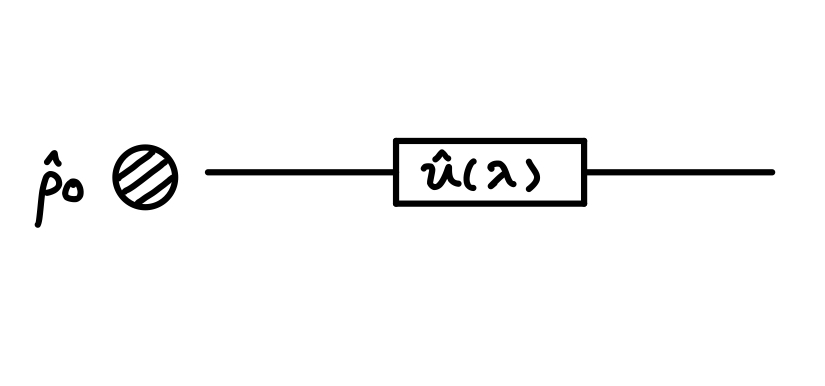
\includegraphics[width=0.90\linewidth]{Single-Particle-QFI.jpg}
\caption{Schematic of Single Particle Unitary Evolution.}
\end{center}
\end{figure}\newpage
At its highest the Quantum Fisher Information will be one for a pure state. As the initial state becomes more and more noisy, i.e the $r$ value gets smaller and smaller the Quantum Fisher Information will decrease. This result shows that for a single particle the best parameter estimation will come from pure states where $r=1$. We can now do the same sort of calculation for multiple noisy particles. 

Take for instance the unitary operator
%--------------------------------------------------
%	Equation (77)
%--------------------------------------------------
\begin{equation} \label{eq:77}
\hat{U}(\lambda)=
\left(\begin{array}{cccc}
e^{-i\lambda/2} & 0 & 0 & 0 \\
0 & e^{-i\lambda/2} & 0 & 0 \\
0 & 0 & e^{i\lambda/2} & 0 \\
0 & 0 & 0 & e^{i\lambda/2} \\
\end{array}\right)
\end{equation}
that acts on the density operator
%--------------------------------------------------
%	Equation (78)
%--------------------------------------------------
\begin{equation} \label{eq:78}
\hat{\rho}=\frac{1}{16}
\left(\begin{array}{cccc}
4+4r^2 & 0 & 0 & -8ir \\
0 & 4-4r^2 & 0 & 0 \\
0 & 0 & 4-4r^2 & 0 \\
8ir & 0 & 0 & 4+4r^2 \\
\end{array}\right).
\end{equation}
We can calculate the Quantum Fisher Information for a two particle system in a similar manner of the single particle system. The only difference is that there is $4x4$ matrix that actually consists of two $2x2$ matrices. So we just have to calculate the Quantum Fisher Information of each matrix and then add them together. When the matrix in equation (\ref{eq:77}) acts on the matrix in (\ref{eq:78}) the Quantum Fisher Information comes out to be
%--------------------------------------------------
%	Equation (79)
%--------------------------------------------------
\begin{equation} \label{eq:79}
H=\frac{2r^2}{1+r^2}.
\end{equation}
The depiction of this measurement can be seen in Figure 5.
%--------------------------------------------------
%	Figure 5
%--------------------------------------------------
\begin{figure}[htpb]
\begin{center}
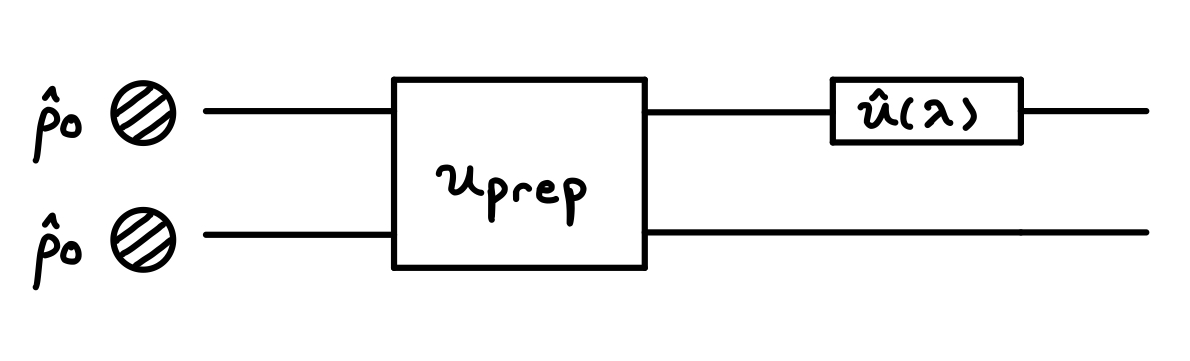
\includegraphics[width=0.90\linewidth]{Two-Particle-One-Unitary-QFI.jpg}
\caption{Schematic of Two Particle Unitary Evolution.}
\end{center}
\end{figure}\\
When we compare the single particle result to the two particle result for very noisy states the two particle state has twice the Quantum Fisher Information. Once again though the two particle system is more accurate in estimating the parameter compared to that of the single particle system. The results can also be improved with entangled states compared to that of the product states.
%---------------------------------------------------------------------------
%	Modeling of Noise
%---------------------------------------------------------------------------
\section*{Modeling of Noise}
In this section we will be discussing the modeling of noise and the evolution that they have on density operators. This evolution can be calculated via
%--------------------------------------------------
%	Equation (80)
%--------------------------------------------------
\begin{equation} \label{eq:80}
\hat{\rho}_f=(1-\alpha)\hat{\rho}_i+\alpha\hspace{1pt}\hat{\sigma}_z\hat{\rho}_i\hat{\sigma}_z
\end{equation}
where $\alpha$ is a parameter between zero and one. This phenomenon is called a phase flip and rotates the particle around the $z$ axis. For particles that are originally oriented in the $+z$ and $-z$ directions there is no change in orientation. If we examine a particle originally oriented in the $+x$ direction with a density operator 
%--------------------------------------------------
%	Equation (81)
%--------------------------------------------------
\begin{equation} \label{eq:81}
\hat{\rho}=\frac{1}{2}
\begin{pmatrix}
1 & 1 \\
1 & 1
\end{pmatrix},
\end{equation}
the evolution of this operator comes out to be
%--------------------------------------------------
%	Equation (82)
%--------------------------------------------------
\begin{equation} \label{eq:82}
\hat{\rho}=\frac{1}{2}
\begin{pmatrix}
1 & 1-2\alpha \\
1-2\alpha & 1
\end{pmatrix}.
\end{equation}
This operator can also be written in the form
%--------------------------------------------------
%	Equation (83)
%--------------------------------------------------
\begin{equation} \label{eq:83}
\hat{\rho}=\frac{1}{2}\big(\hat{I}+(1-2\alpha)\hat{\sigma}_x\big).
\end{equation}
If we examine another initial direction for how noise evolves a particle, say the $-y$ direction with the density operator of 
%--------------------------------------------------
%	Equation (84)
%--------------------------------------------------
\begin{equation} \label{eq:84}
\hat{\rho}=\frac{1}{2}
\begin{pmatrix}
1 & i \\
-i & 1
\end{pmatrix}
\end{equation}
originally, the evolution of this operator under equation (\ref{eq:80}) comes out to be
%--------------------------------------------------
%	Equation (85)
%--------------------------------------------------
\begin{equation} \label{eq:85}
\hat{\rho}=\frac{1}{2}
\begin{pmatrix}
1 & i(1-2\alpha) \\
i(2\alpha-1) & 1
\end{pmatrix}.
\end{equation}
This final density operator can be written in the form of 
%--------------------------------------------------
%	Equation (86)
%--------------------------------------------------
\begin{equation} \label{eq:86}
\hat{\rho}=\frac{1}{2}\big(\hat{I}+(2\alpha-1)\hat{\sigma}_y\big).
\end{equation}
These calculations are vital for understanding how particles evolve in certain systems when we are trying to obtain measurement estimates. 

Consider a particle originally in the $\hat{\rho}=\ket{0}\bra{0}$ state. The evolution of this particle according to equation (\ref{eq:80}) comes out to be
%--------------------------------------------------
%	Equation (87)
%--------------------------------------------------
\begin{equation} \label{eq:87}
\hat{\rho}=
\begin{pmatrix}
1 & 0 \\
0 & 0
\end{pmatrix}.
\end{equation}
We can observe that this particle does not encounter a change in orientation, the same can be said for the particle originally in the $\hat{\rho}=\ket{1}\bra{1}$ state where the evolution of this operator under equation (\ref{eq:80}) comes out to be
%--------------------------------------------------
%	Equation (88)
%--------------------------------------------------
\begin{equation} \label{eq:88}
\hat{\rho}=
\begin{pmatrix}
0 & 0 \\
0 & 1
\end{pmatrix}.
\end{equation}
Evolutions of these states occur for the $\hat{\rho}=\ket{0}\bra{1}$ state which comes out to be
%--------------------------------------------------
%	Equation (89)
%--------------------------------------------------
\begin{equation} \label{eq:89}
\hat{\rho}=
\begin{pmatrix}
0 & 1-2\alpha \\
0 & 0
\end{pmatrix}.
\end{equation}
Lastly, the state $\hat{\rho}=\ket{1}\ket{0}$ evolves to 
%--------------------------------------------------
%	Equation (90)
%--------------------------------------------------
\begin{equation} \label{eq:90}
\hat{\rho}=
\begin{pmatrix}
0 & 0 \\
1-2\alpha & 0
\end{pmatrix}
\end{equation}
again under equation (\ref{eq:80}). For the evolutions described in ($\ref{eq:87}$) - ($\ref{eq:90}$) we will have different evolutions for different $\hat{\sigma}$'s in equation ($\ref{eq:80}$).
%---------------------------------------------------------------------------
%	Quantum Fisher Information Involving Phase Flips
%---------------------------------------------------------------------------
\section*{Quantum Fisher Information Involving Phase Flips}
Now that we have an understanding of how we model noise we can move on to estimating parameters in these situations where noise exist. Using the density operator in equation (\ref{eq:77}) and the unitary operator in equation (\ref{eq:78}) we wish to examine how good of an estimation procedure this is. With this scenario, one particle is being influence by the unitary operator and the other is undergoing a phase flip defined by equation (\ref{eq:80}). When we run through the mechanics of this calculation the Quantum Fisher Information is
%--------------------------------------------------
%	Equation (91)
%--------------------------------------------------
\begin{equation}\label{eq:91}
H=\frac{2r^2(1-2\alpha)^2}{(1+r^2)}.
\end{equation}
This measurement can be seen in Figure 6.
%--------------------------------------------------
%	Figure 6
%--------------------------------------------------
\begin{figure}[htpb]
\begin{center}
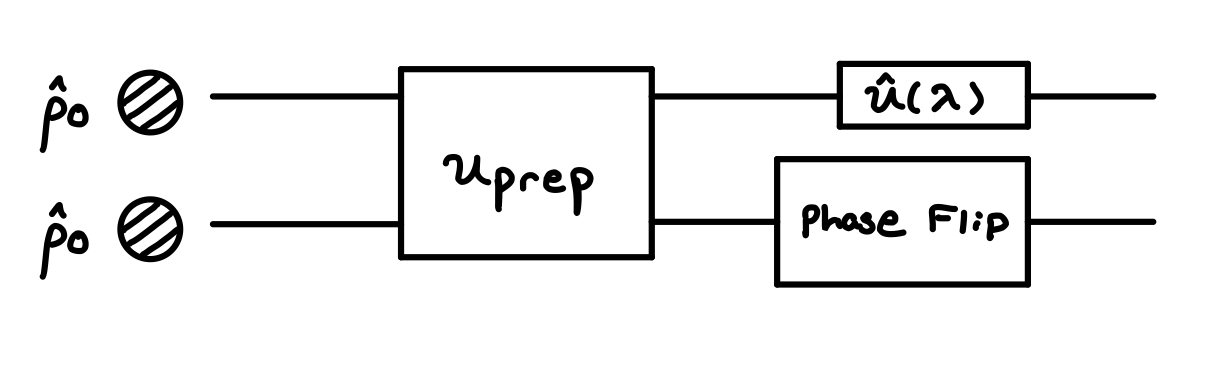
\includegraphics[width=0.90\linewidth]{Two-Particle-Phase-Flip.jpg}
\caption{Schematic of Two Particle Phase Flip Evolution.}
\end{center}
\end{figure}\\
The $\alpha$ value in equation (\ref{eq:80}) defines how noisy our state is. If $\alpha=0$ then the state is not noisy at all and it is pure. If $\alpha=1$ then the state is very noisy. When we examine the extremes of this scenario, i.e $\alpha=0$ or $\alpha=1$ we have the Quantum Fisher Information in equation (\ref{eq:79}). When $\alpha=1/2$ the Quantum Fisher Information is 0 and the parameter cannot be estimated.

We can examine the same scenario but instead of $\hat{\sigma}_z$ in equation (\ref{eq:80}) we will examine a bit flip with $\hat{\sigma}_x$. When this scenario is examined and the calculation is made, the Quantum Fisher Information is
%--------------------------------------------------
%	Equation (92)
%--------------------------------------------------
\begin{equation}\label{eq:92}
H=\frac{2r^2\alpha^2}{((2\alpha-1)r^2+1)}+\frac{2r^2(1-\alpha)^2}{(1-(2\alpha-1)r^2)}.
\end{equation}
When we examine the same extreme scenarios we still get the result in equation (\ref{eq:79}).
%---------------------------------------------------------------------------
%	Conclusion
%---------------------------------------------------------------------------
\section*{Conclusion}
It has been observed so far that entangled states produce the best estimates to physical parameters. Along with that, pure states yield better measurements compared to that of noisy states. Along with entangled states, more states that are involved in the measurement process produce better estimates to parameters. The relationship for the Quantum Fisher Information is $H=n$ for pure product states and $H=n^2$ for pure entangled states. The Quantum Fisher Information for noisy states is dependent upon how noisy the states are that are being measured. With very noisy or pure states the Quantum Fisher Information will reduce to that of equation (\ref{eq:79}) for the scenarios that have been covered in this article.
%---------------------------------------------------------------------------
%	Bibliography
%---------------------------------------------------------------------------
\newpage
\begin{thebibliography}{99}
\bibitem{D. Collins}
Collins, D. (2019). Qubit-channel metrology with very noisy initial states. Physical Review A, 99(1). doi: 10.1103/physreva.99.012123
\bibitem{Fisher Information}
Fisher Information. (2019, October 11). Retrieved November 13, 2019, from \url{https://en.wikipedia.org/wiki/Fisher_information.}
\bibitem{Spherical Coordinates}
Spherical coordinate system. (2019, August 6). Retrieved from \url{https://en.wikipedia.org/wiki/Spherical_coordinate_system#/media/File:3D_Spherical.svg}
\end{thebibliography}
%-----------------------------------------------------------------------------------------------------------------------------
%	End Document
%-----------------------------------------------------------------------------------------------------------------------------
\end{document}
%---------------------------------------------------------------------------
%	Comment Headers
%---------------------------------------------------------------------------

%---------------------------------------------------------------------------
%	
%---------------------------------------------------------------------------

%--------------------------------------------------
%	
%--------------------------------------------------
